\setmainfont{Noto Serif}
\setsansfont{Noto Sans}
\setmonofont{Noto Sans Mono}
\setstretch{1.35}


%\phantomsection
\section{Описание электронного строения атомов и молекул}
%\addcontentsline{toc}{chapter}{1 Описание электронного строения атомов и молекул}
%\markboth{Описание электронного строения атомов и молекул}{Описание электронного строения атомов и молекул}
\subsection{Угловой момент. Сложение моментов}
1. 1 \\
2. 2 
\newpage

\subsection{Термы многоэлектронных атомов}
1. 1 \\
2. 2
\newpage

\subsection{Дипольные переходы между термами}
1. Задача 2 контрольной работы 1 осеннего семестра 2023/2024 учебного года. Не равна нулю только $d_z$ компонента вектора $\vec d$. Она равна $3ea_0/Z$, где $a_0$ – радиус Бора, $Z$ – заряд ядра. Величина электрического дипольного момента перехода совпадает с $d_z$.\par
2. Задача 3 контрольной работы 1 осеннего семестра 2023/2024 учебного года. Основной мультиплет $^3H_4$. Электические дипольные переходы возможны в~мультиплеты $^3G_3$, $^3F_{3,2}$, $^3D_{3,2,1}$. Возбужденная электронная конфигурация должна быть четной.\par
3. Задача 5 контрольной работы 1 осеннего семестра 2024/2025 учебного года.  Полное количество термов 47. Основной терм $^5I$. Переход возможен в любую нечетную электронную конфигурацию, например, $6s^14f^46p^1$.\par
4. Задача 3 контрольной работы 1 осеннего семестра 2024/2025 учебного года. Всего 18 переходов. Условию удовлетворяют переходы $^3P\, \rightarrow\, ^3P$ и переходы $^3P\, \rightarrow\, ^3D$. Всего их 7 штук.\par
5. Задача 5 контрольной работы 1 осеннего семестра 2023/2024 учебного года. Серия А относится к переходу (1). Серия B относится к переходу (2). Серия C~относится к переходу (1).   \\
\newpage

\subsection{Многоэлектронный атом во внешних полях}
1. 1 \\
2. 2 \\
4. Задача 4 контрольной работы 1 осеннего семестра 2024/2025 учебного года. Эффективная константа спин-орбитального взаимодействия $\lambda$ равна 0,12 см$^{-1}$, индукция магнитного поля $B$ равна 2,014 Тл.\par
\newpage

\subsection{Правила Вигнера-Витмера}
1. Независимых волновых функций: 1 ($^1\Sigma^-$), 3 ($\,^3\Sigma^+$), 6 ($\,^3\Pi$), 2 ($^1\Phi$), 12~($^6\Delta$). \par
2.  $^{6,4,2}\Pi$,  $^{6,4,2}\Sigma^+$.\par
3. (1) $^3\Delta_u$, $^1\Delta_g$, $^{3,1}\Pi_g$, $^{3,1}\Pi_u$, $2 \times ^{3}\Sigma_u^+$, $^3\Sigma^-_g$, $2 \times ^{1}\Sigma_g^+$, $^{1}\Sigma_u^-$; (2) $^{3,1}\Pi_g$, $^{3,1}\Pi_u$, $^{3,1}\Sigma^-_g$, $^{3,1}\Sigma^-_u$; (3)~$^3\Pi_g$, $^3\Pi_u$, $^3\Sigma^-_g$, $^3\Sigma^-_u$.\par
4. $(2S_2+1)(2L_2+1)(L_1+1).$\par
5.  $^{5}\Sigma^+$, $3 \times ^{3}\Sigma^+$, $2 \times ^{1}\Sigma^+$.\par
6. Задача 2 контрольной работы 1 осеннего семестра 2021/2022 учебного года. Термы: $^3\Pi$, $^3\Sigma^-$. Основного состояния молекулы BeO получиться не может. Для образования BeO в основном электронном состоянии нужно, например, возбужденное состояние атома бериллия $^3P$, соответствующее электронной конфигурации $2s^12p^1$.\par
7. Задача 2 контрольной работы 2 осеннего семестра 2024/2025 учебного года. Реакция протекает по гомолитическому механизму.\par
8. Образование CO в основном состоянии в этом случае возможно.\par
9. $^1\Delta_g$, $^1\Pi_g$, $^1\Pi_u$, $2 \times ^1\Sigma^+_g$, $^1\Sigma^-_u$.\par
10. $1 + LS + S + L(2 + L + 2(1 + L)S)$\par
\newpage

\subsection{Электронное строение двухатомных молекул}
1. 1 \\
2. 2
\newpage

\subsection{Электронное строение многоатомных молекул}
1. 1 \\
2. 2
\newpage

\subsection{Специальные хюккелевские системы}
1. 1 \\
2. 2
\newpage

\subsection{Применение теории возмущений}
1. 1 \\
2. 2
\newpage

%\usepackage[fit, breakall]{truncate}
%\phantomsection
\section[Спектроскопические методы исследования вещества]{\texorpdfstring{Электронное строение координационных соединений.\\Спектроскопические методы исследования вещества}{Электронное строение координационных соединений. Спектроскопические методы исследования вещества}}
%\addcontentsline{toc}{chapter}{2 Электронное строение координационных соединений. Спектроскопические методы исследования }
%\markboth{Электронное строение координационных соединений. Спектроскопические методы исследования}{Электронное строение координационных соединений. Спектроскопические методы исследования}
\subsection{Правила Вудворда-Хоффмана}
\begin{wrapfigure}{r}{30mm} %this figure will be at the right
    \centering
    \vspace{1.8mm}
    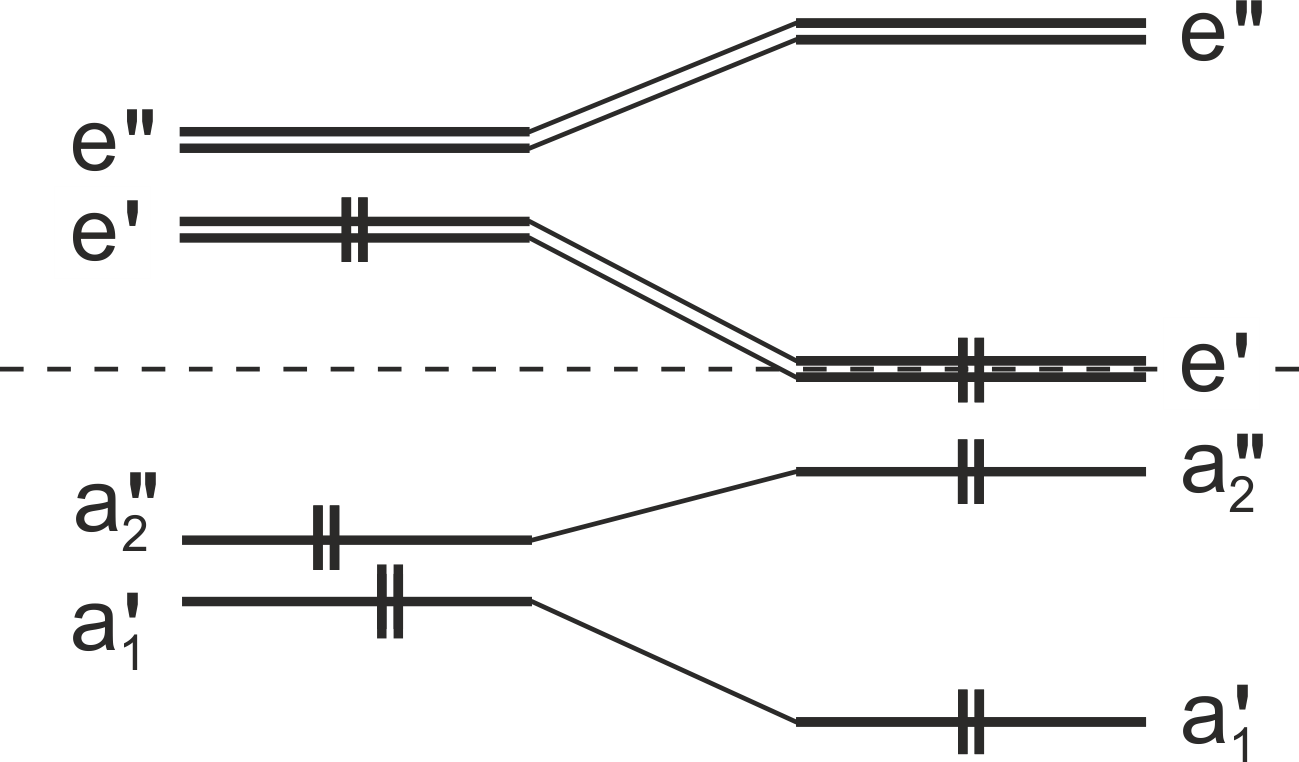
\includegraphics[width=30mm]{images/Fig_2_1_1_dec.png}
    \vspace{-5mm}
\end{wrapfigure}
1. Задача 3 контрольной работы 1 весеннего семестра 2021/2022 учебного года. Корреляционная диаграмма для группы симметрии $D_{3h}$ приведена на рисунке ниже.  Считая, что в реагентах молекулярные орбитали с симметрией $a'_1$ и $a''_2$, а также орбитали $e'$ и $e''$ имеют одинаковую энергию, изменение полной электронной энергии равно $2\beta$. Реакция разрешена термически.\par
\begin{wrapfigure}{r}{30mm} %this figure will be at the right
    \centering
    \vspace{-2.2mm}
    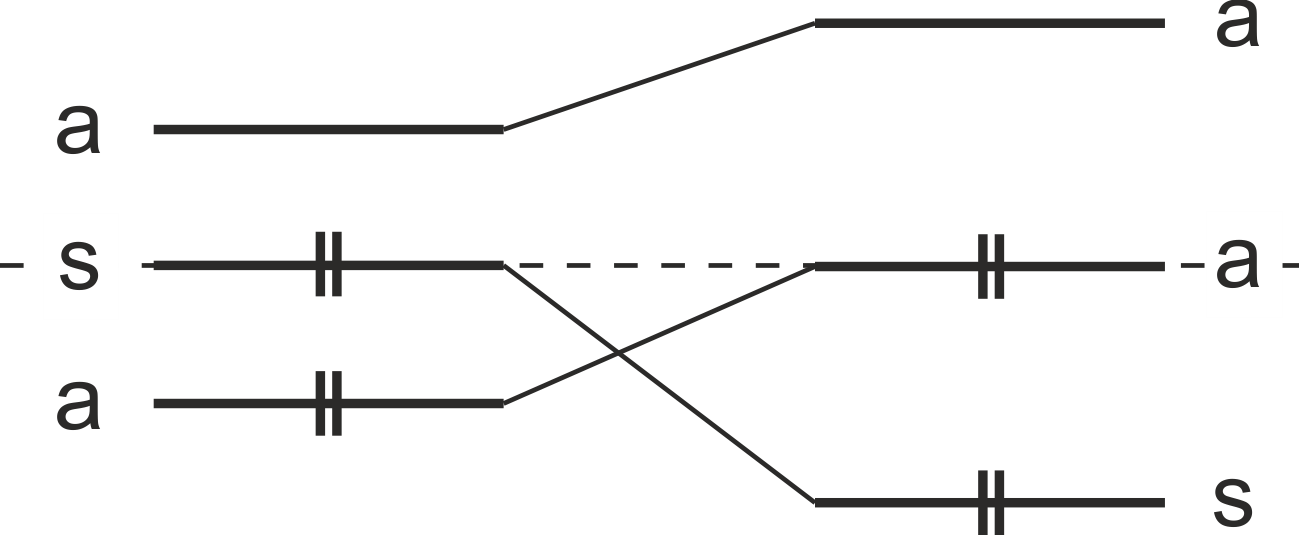
\includegraphics[width=30mm]{images/Fig_2_1_2_dec.png}
    \vspace{-5mm}
\end{wrapfigure}
2. Задача 1 контрольной работы 1 весеннего семестра 2023/2024 учебного года. Данная реакция термически протекает в конротаторном механизме, поэтому продуктом является цис-изомер, соответствующая корреляционная диаграмма приведена на рисунке.\par
3. В ходе реакции сохраняется группа симметрии $C_2$, при этом меняется направление единственной оси симметрии данной группы. Аналогично можно рассмотреть группу симметрии $D_2$. Реакция запрещена термически. Связывающая молекулярная орбиталь (МО) реагентов симметрии $b$ в базисе $2p_z$ атомных орбиталей становится разрыхляющей орбиталью продуктов, разрыхляющая МО реагентов симметрии $a$ становится связывающей орбиталью продуктов.\par
4. В $4\pi_s$ + $2\pi_s$ топологии реакция разрешена термически, есть ровно один $4n+2$ супра-компонент. В супра-/антара- топологии реакция запрещена термически, так как она соответствует, например, $2\pi_s$ + $2\pi_s$ + $2\pi_a$ компонентам. Корреляционная диаграмма для супра-/супра- топологии приведена на~рисунке. Для случая супра-/антара- топологии корреляционную диаграмму построить нельзя. В ходе реакции не сохраняется ни один элемент симметрии, см. рисунок.\par
\vspace{-\parskip}
\vspace{1mm}
\begin{figure}[h]
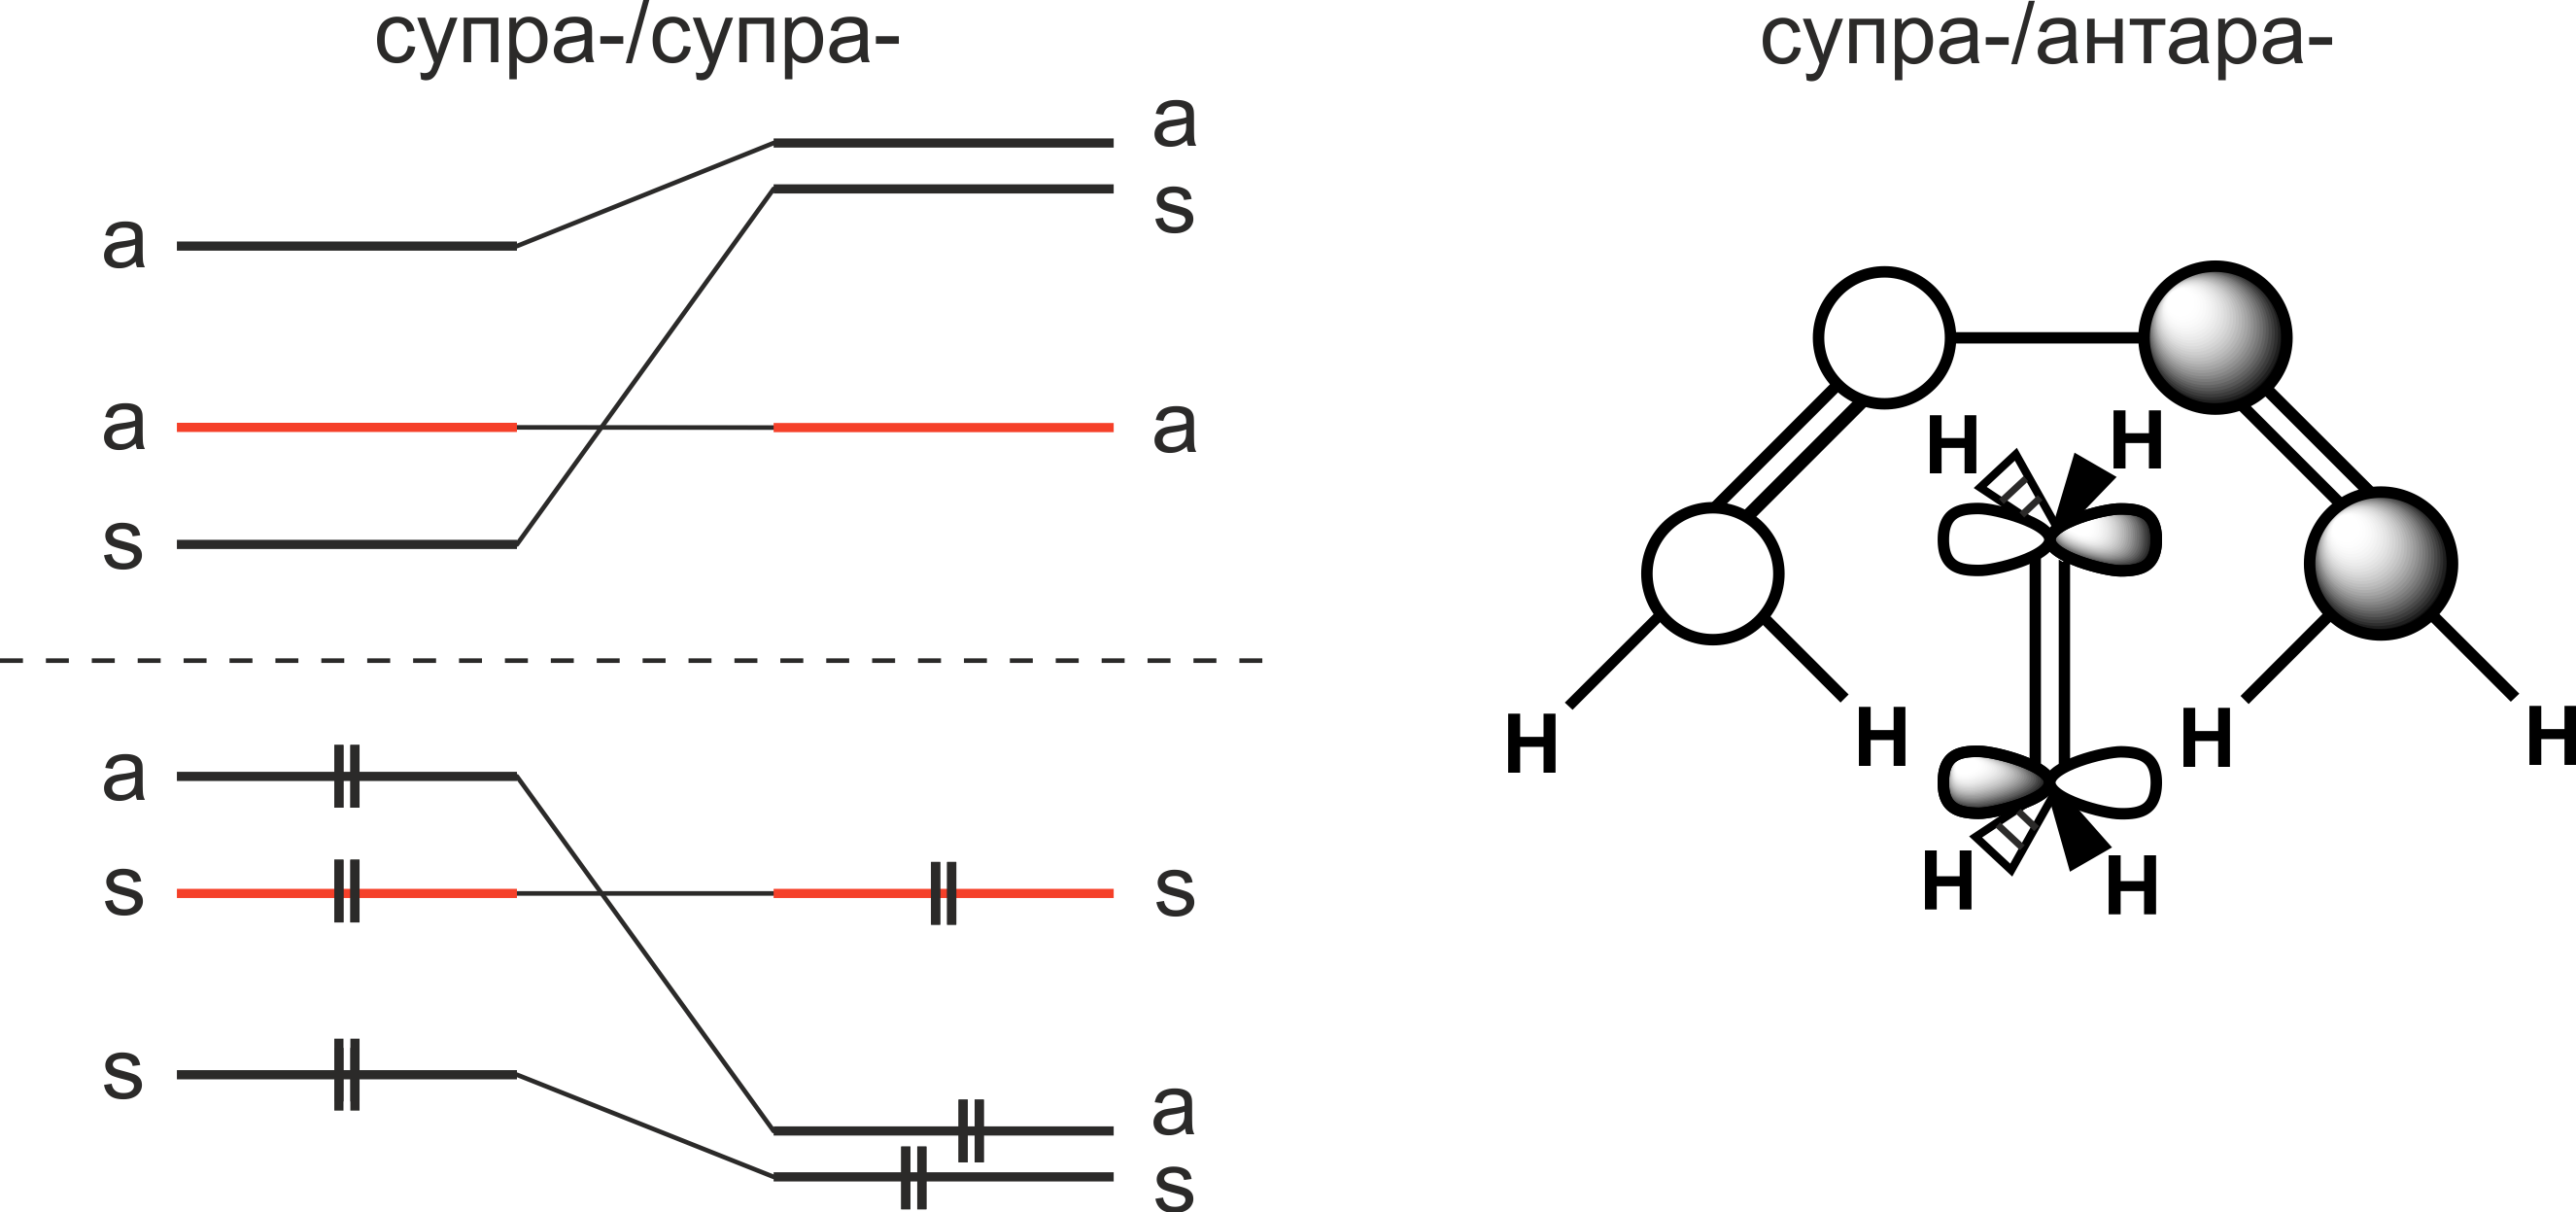
\includegraphics[width=6.5cm]{images/Fig_2_1_4_dec.png}
\centering
\end{figure}
\vspace{-\parskip}
\par
\begin{wrapfigure}{r}{30mm} %this figure will be at the right
    \centering
    \vspace{-0.7mm}
    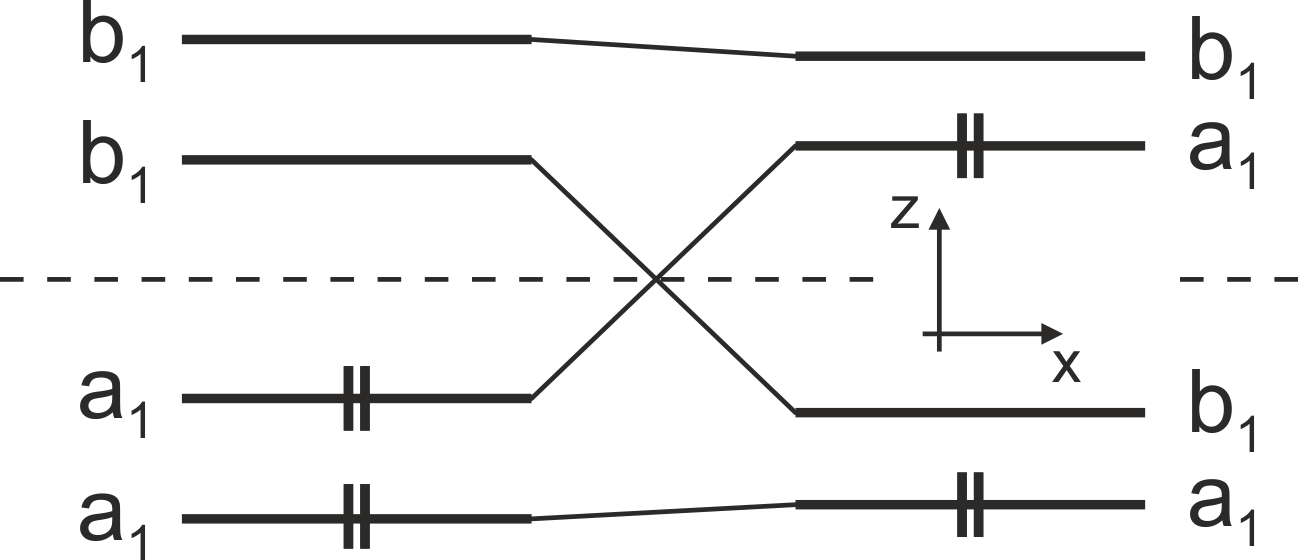
\includegraphics[width=30mm]{images/Fig_2_1_5_dec.png}
    \vspace{-9mm}
\end{wrapfigure}
5. В ходе всей реакции сохраняется группа симметрии  $C_{2v}$. Реакция протекает фотохимически. Корреляционная диаграмма приведена на рисунке.\par
%\vspace{-\parskip}
\begin{wrapfigure}{r}{30mm} %this figure will be at the right
    \centering
    \vspace{5.4mm}
    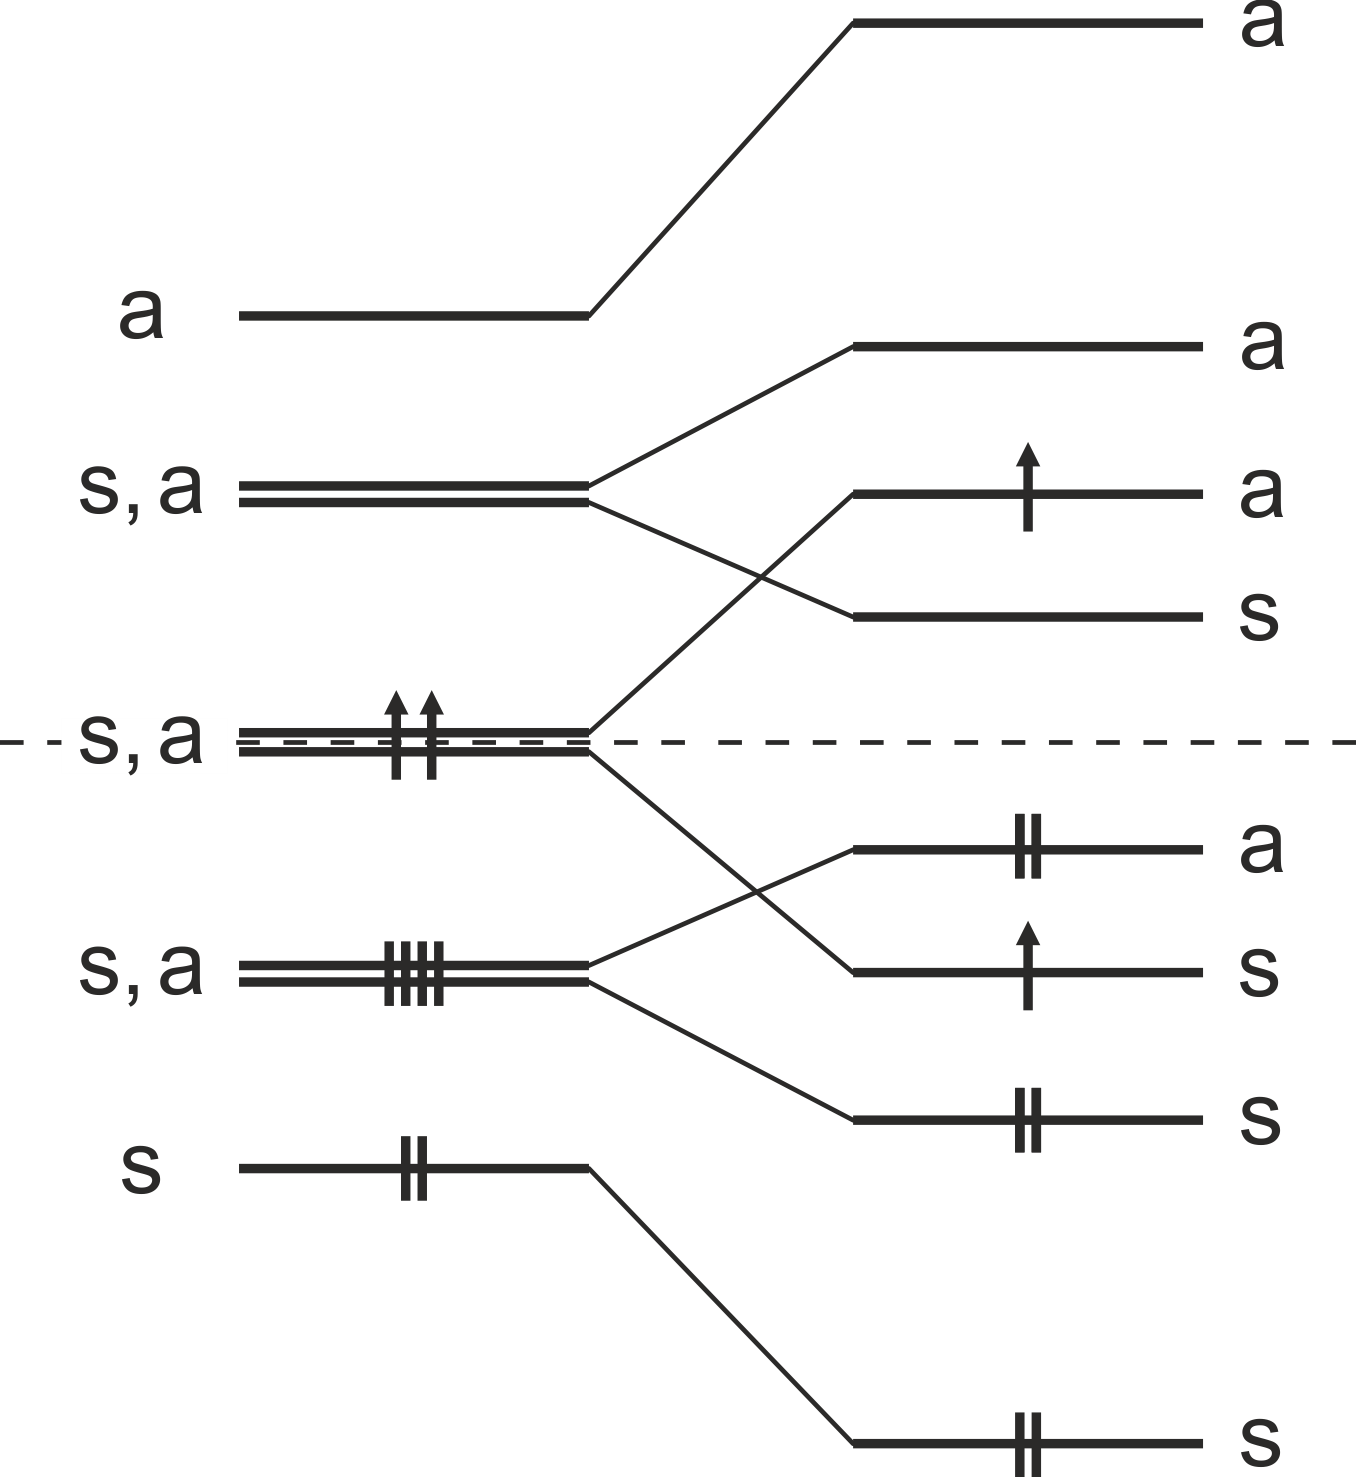
\includegraphics[width=30mm]{images/Fig_2_1_6_dec.png}
    \vspace{-5mm}
\end{wrapfigure}
6. Если считать, что циклооктатетраен плоский, то его основной терм триплетный по спину и реакция запрещена термически для дисротаторного механизма. Корреляционная диаграмма приведена на рисунке. Данный подход не совсем корректный. Если же учесть конформацию циклооктатетраена, необходимую для протекация реакции, то данная реакция в дисротаторном механизме соответствует трем $2\pi_s$ компонентам, то~есть она разрешена термически. В этом случае одна двойная связь выходит из сопряжения и~не участвует в~реакции. Реагент необходимо рассматривать как две линейные $\pi$-системы из 2 и 6 атомов, соответственно.\par
%\vspace{-\parskip}
\begin{wrapfigure}{r}{30mm} %this figure will be at the right
    \centering
    \vspace{-1mm}
    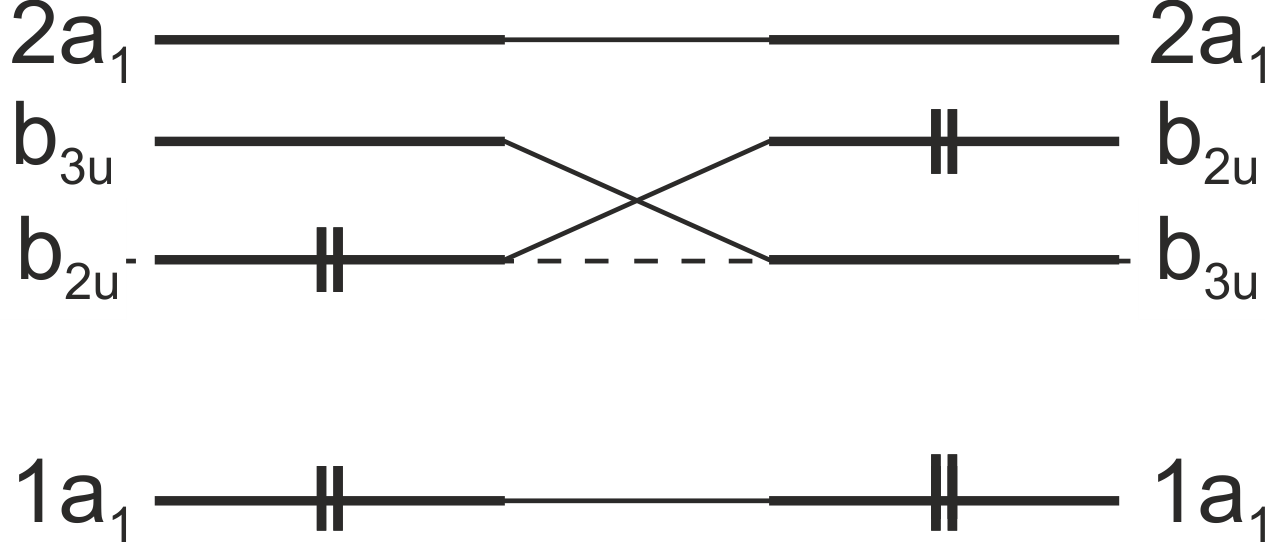
\includegraphics[width=30mm]{images/Fig_2_1_7_dec.png}
    \vspace{-5mm}
\end{wrapfigure}
7. В ходе всей реакции сохраняется группа симметрии $D_{2h}$. Корреляционная диаграмма для указанной в~условии системы координат и базиса $1s$ атомных орбиталей приведена на рисунке, реакция запрещена термически. Изменение полной электронной энергии равно $-2\beta$.\par
%\vspace{-\parskip}
8. Общая формулировка правил Вудворда-Хоффмана: перициклическая реакция термически разрешена если общее число $4n+2$ супраповерхностых и~$4n$~антараповерхностных компонент равно нечетному числу.  Более конкретно для~циклоприсоединения Дильса-Альдера, если $p+q=4n$, то реакция разрешена термически для супра-/антара- и антара-/супра- топологий, разрешена фотохимически для супра-/супра- и антара-/антара- топологий. Если $p+q=4n+2$, то~реакция разрешена термически для супра-/супра- и антара-/антара- топологий, разрешена фотохимически для супра-/антара- и антара-/супра- топологий. В~данном случае $p$ и $q$ равны количеству электронов в $\pi$-системах реагентов, а~$n$~– целое число.\par
%\vspace{-\parskip}
\begin{wrapfigure}{r}{30mm} %this figure will be at the right
    \centering
    \vspace{0mm}
    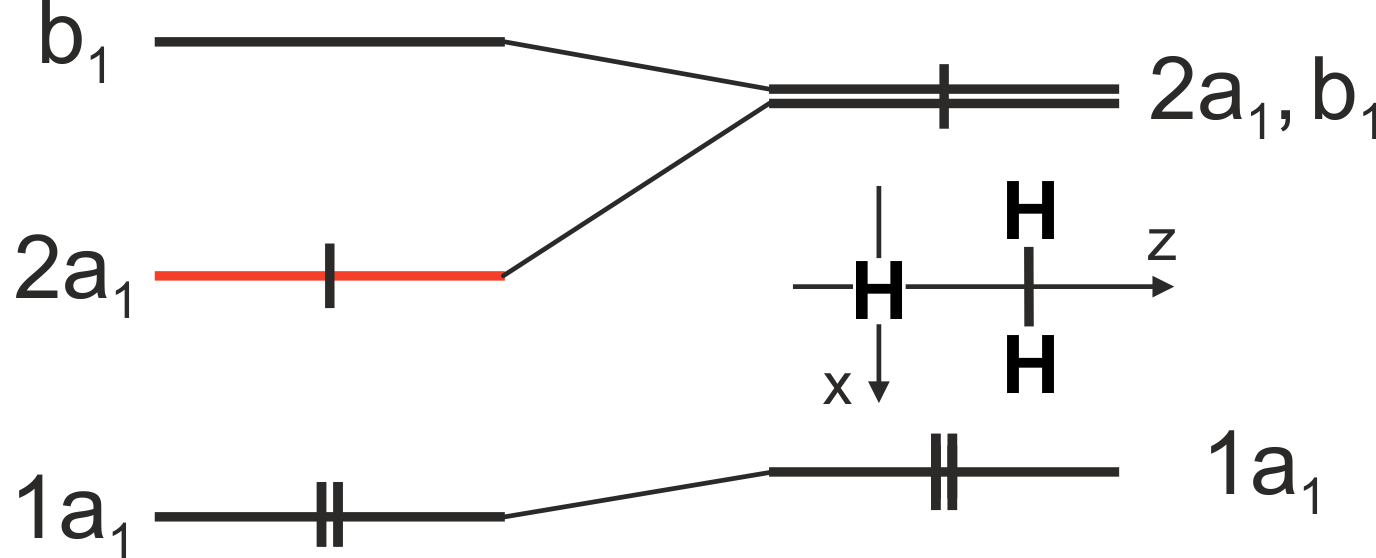
\includegraphics[width=30mm]{images/Fig_2_1_9_dec.png}
    \vspace{-5mm}
\end{wrapfigure}
9. В ходе всей реакции сохраняется группа симметрии $C_{2v}$. Корреляционная диаграмма приведена на рисунке. Реакция разрешена термически. Электрический дипольный переход в~H$_2$ возможен в конфигурацию $a_1^1b_1^1$, терм $^1B_1$. Фотохимически реакция также разрешена.\par
%\vspace{-\parskip}
10. Данная рекция может протекать как через промежуточное состояние в~конформации кресло, так и в конформации ванна. Рассмотрим для определенности только конформацию кресло. Как показано на рисунке, в этом случае реакция соответствует $2\pi_s$ + $2\pi_s$ + $2\sigma_s$ компонентам. Всего три $4n+2$ супра-компоненты, то есть реакция разрешена термически. Стереохимия продукта также приведена на рисунке. В случае конформации ванна данная реакция также разрешена термически.\par
\vspace{-\parskip}
\vspace{1mm}
\begin{figure}[h]
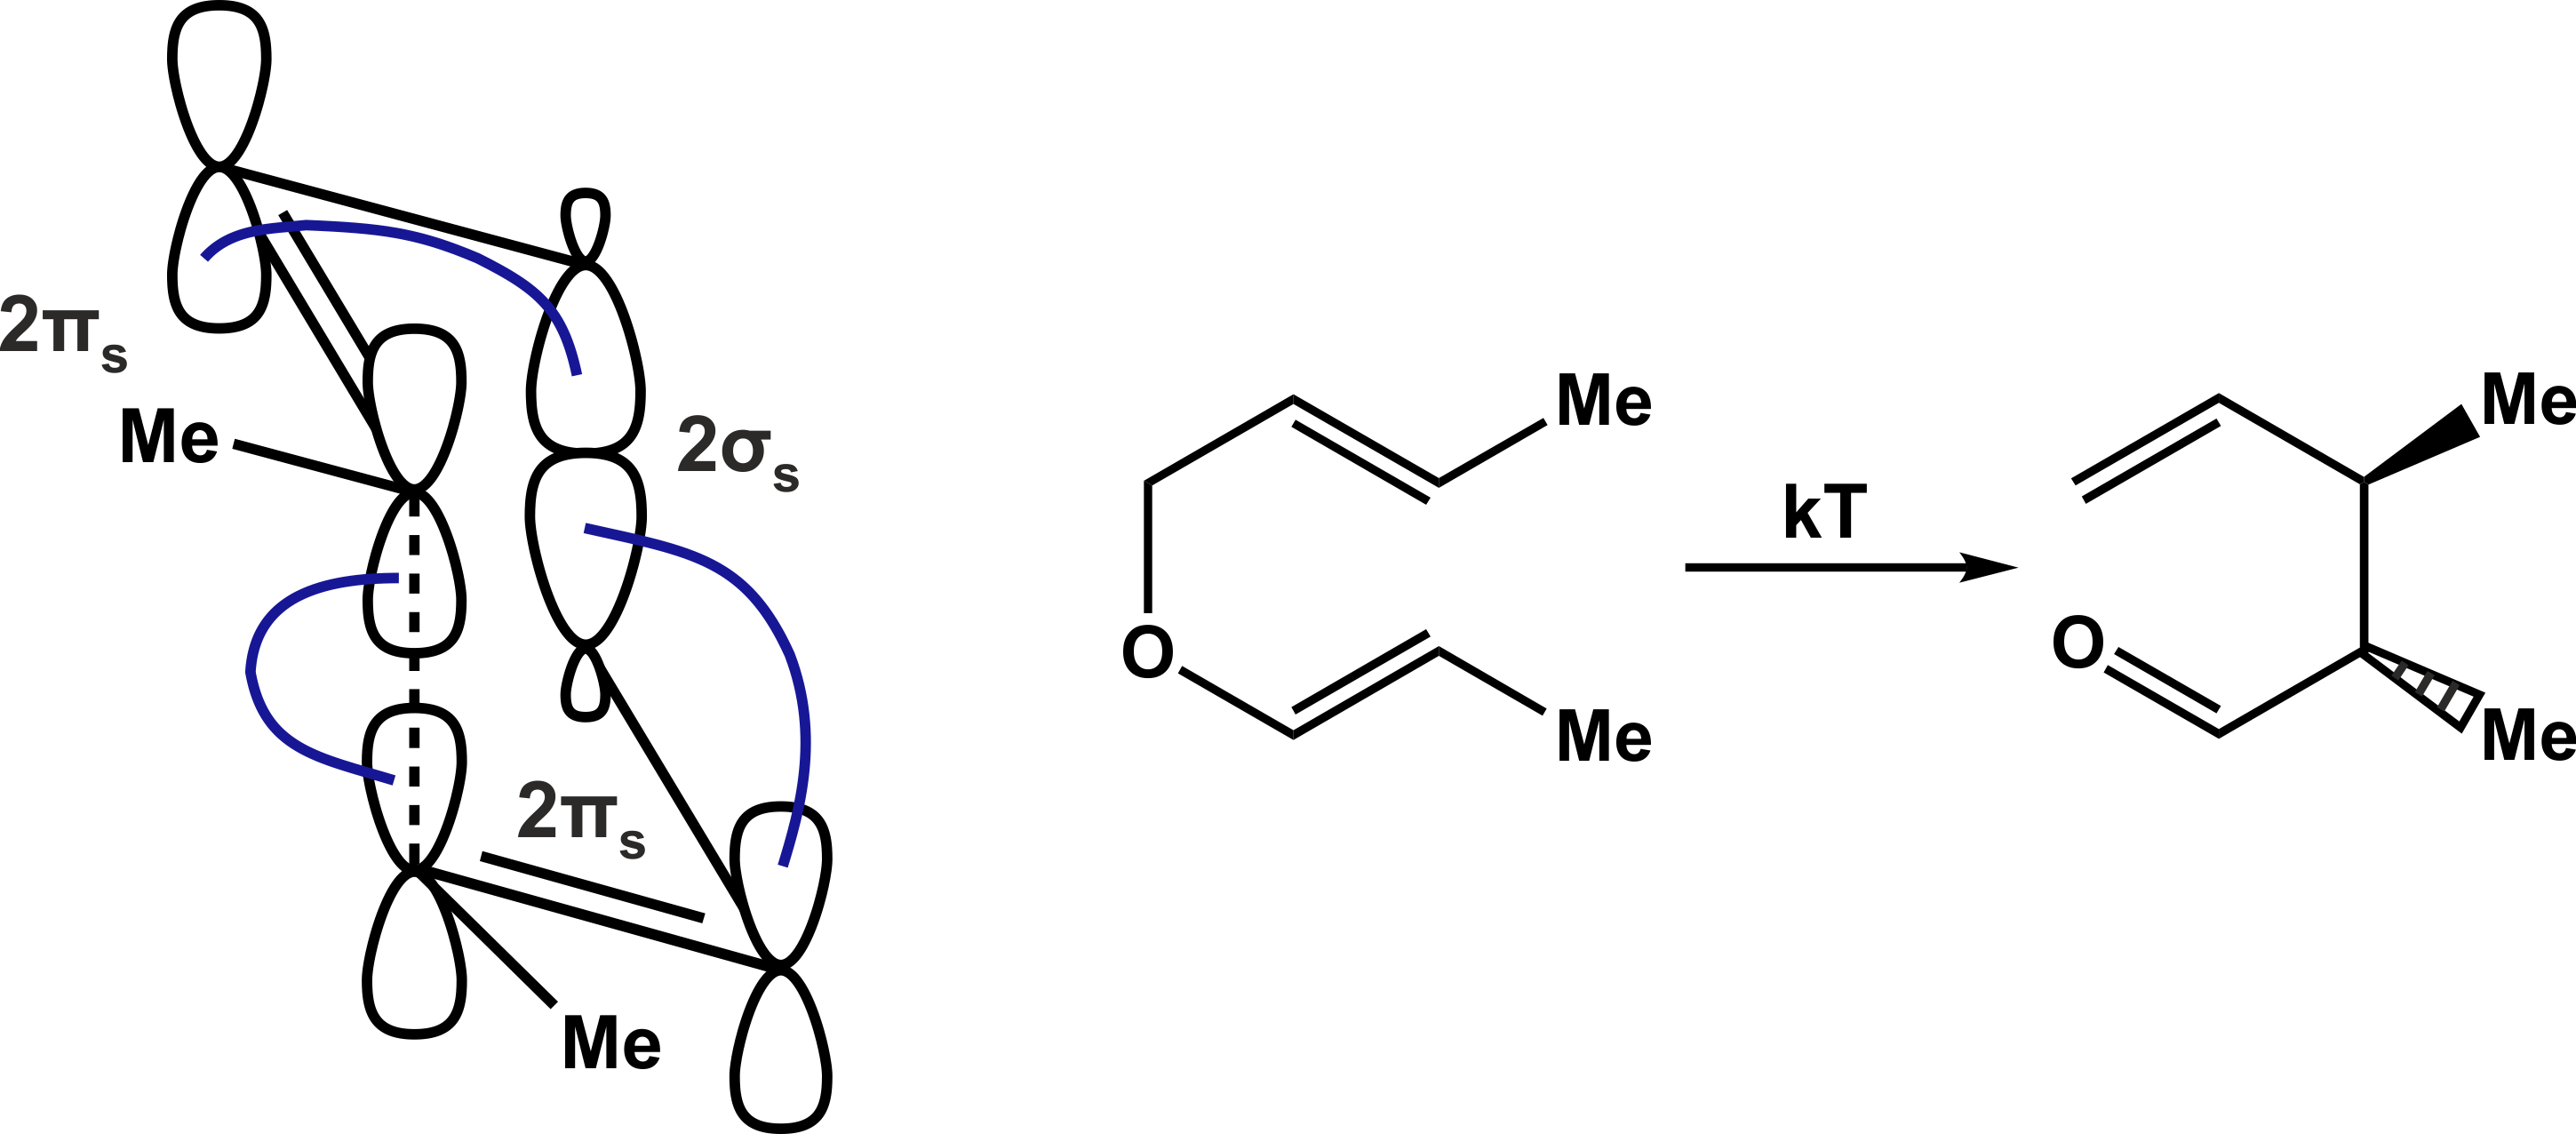
\includegraphics[width=6.5cm]{images/Fig_2_1_10_dec.png}
\centering
\end{figure}
\par
%\vspace{-\parskip}
\vspace{-\parskip}
\begin{wrapfigure}{r}{30mm} %this figure will be at the right
    \centering
    \vspace{4mm}
    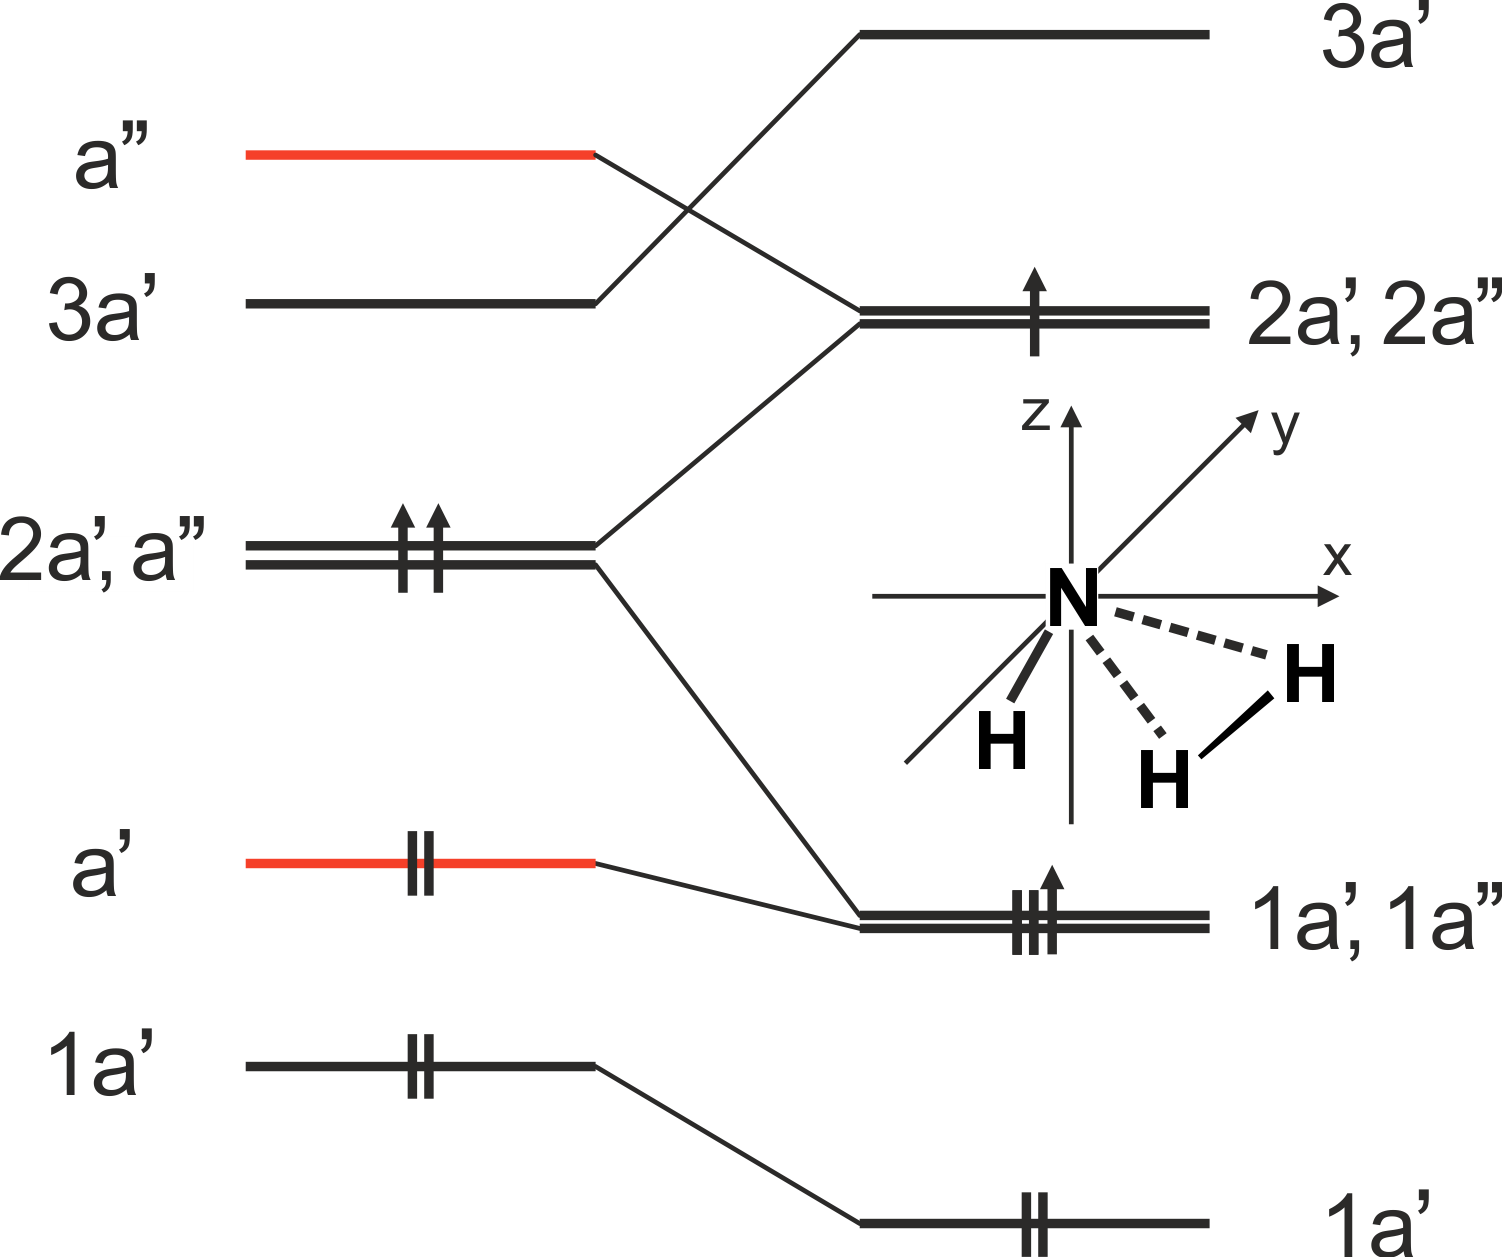
\includegraphics[width=30mm]{images/Fig_2_1_11_dec.png}
    \vspace{-5mm}
\end{wrapfigure}
11. В ходе всей реакции сохраняется группа симметрии $C_s$ с единственной операцией симметриии $\sigma_{zx}$. Корреляционная диаграмма приведена на рисунке. Для простоты для атома азота учитываются только $2p$ атомные орбитали. Расположение молекулярных орбиталей по~энергии приведено качественно. Молекулярные орбитали молекулы водорода выделены красным цветом. Основное триплетное состояние реагентов коррелирует с возбужденным состоянием молекулы аммиака. Реакция запрещена термически.\par
12. Считаем, что при таком протекании реакции $3d$ атомные орбитали металла включены в систему молекулярных орбиталей. Их расщепление в поле двух этиленов для простоты не учитываем. В ходе всей реакции сохраняется группа симметрии $C_{2v}$. Корреляционная диаграмма приведена на рисунке. Реакция термически разрешена для электронных конфигураций $3d^2-3d^8$, без учета спиновой мультиплетности основного терма металла.\par
\vspace{-\parskip}
\vspace{1.5mm}
\begin{figure}[h]
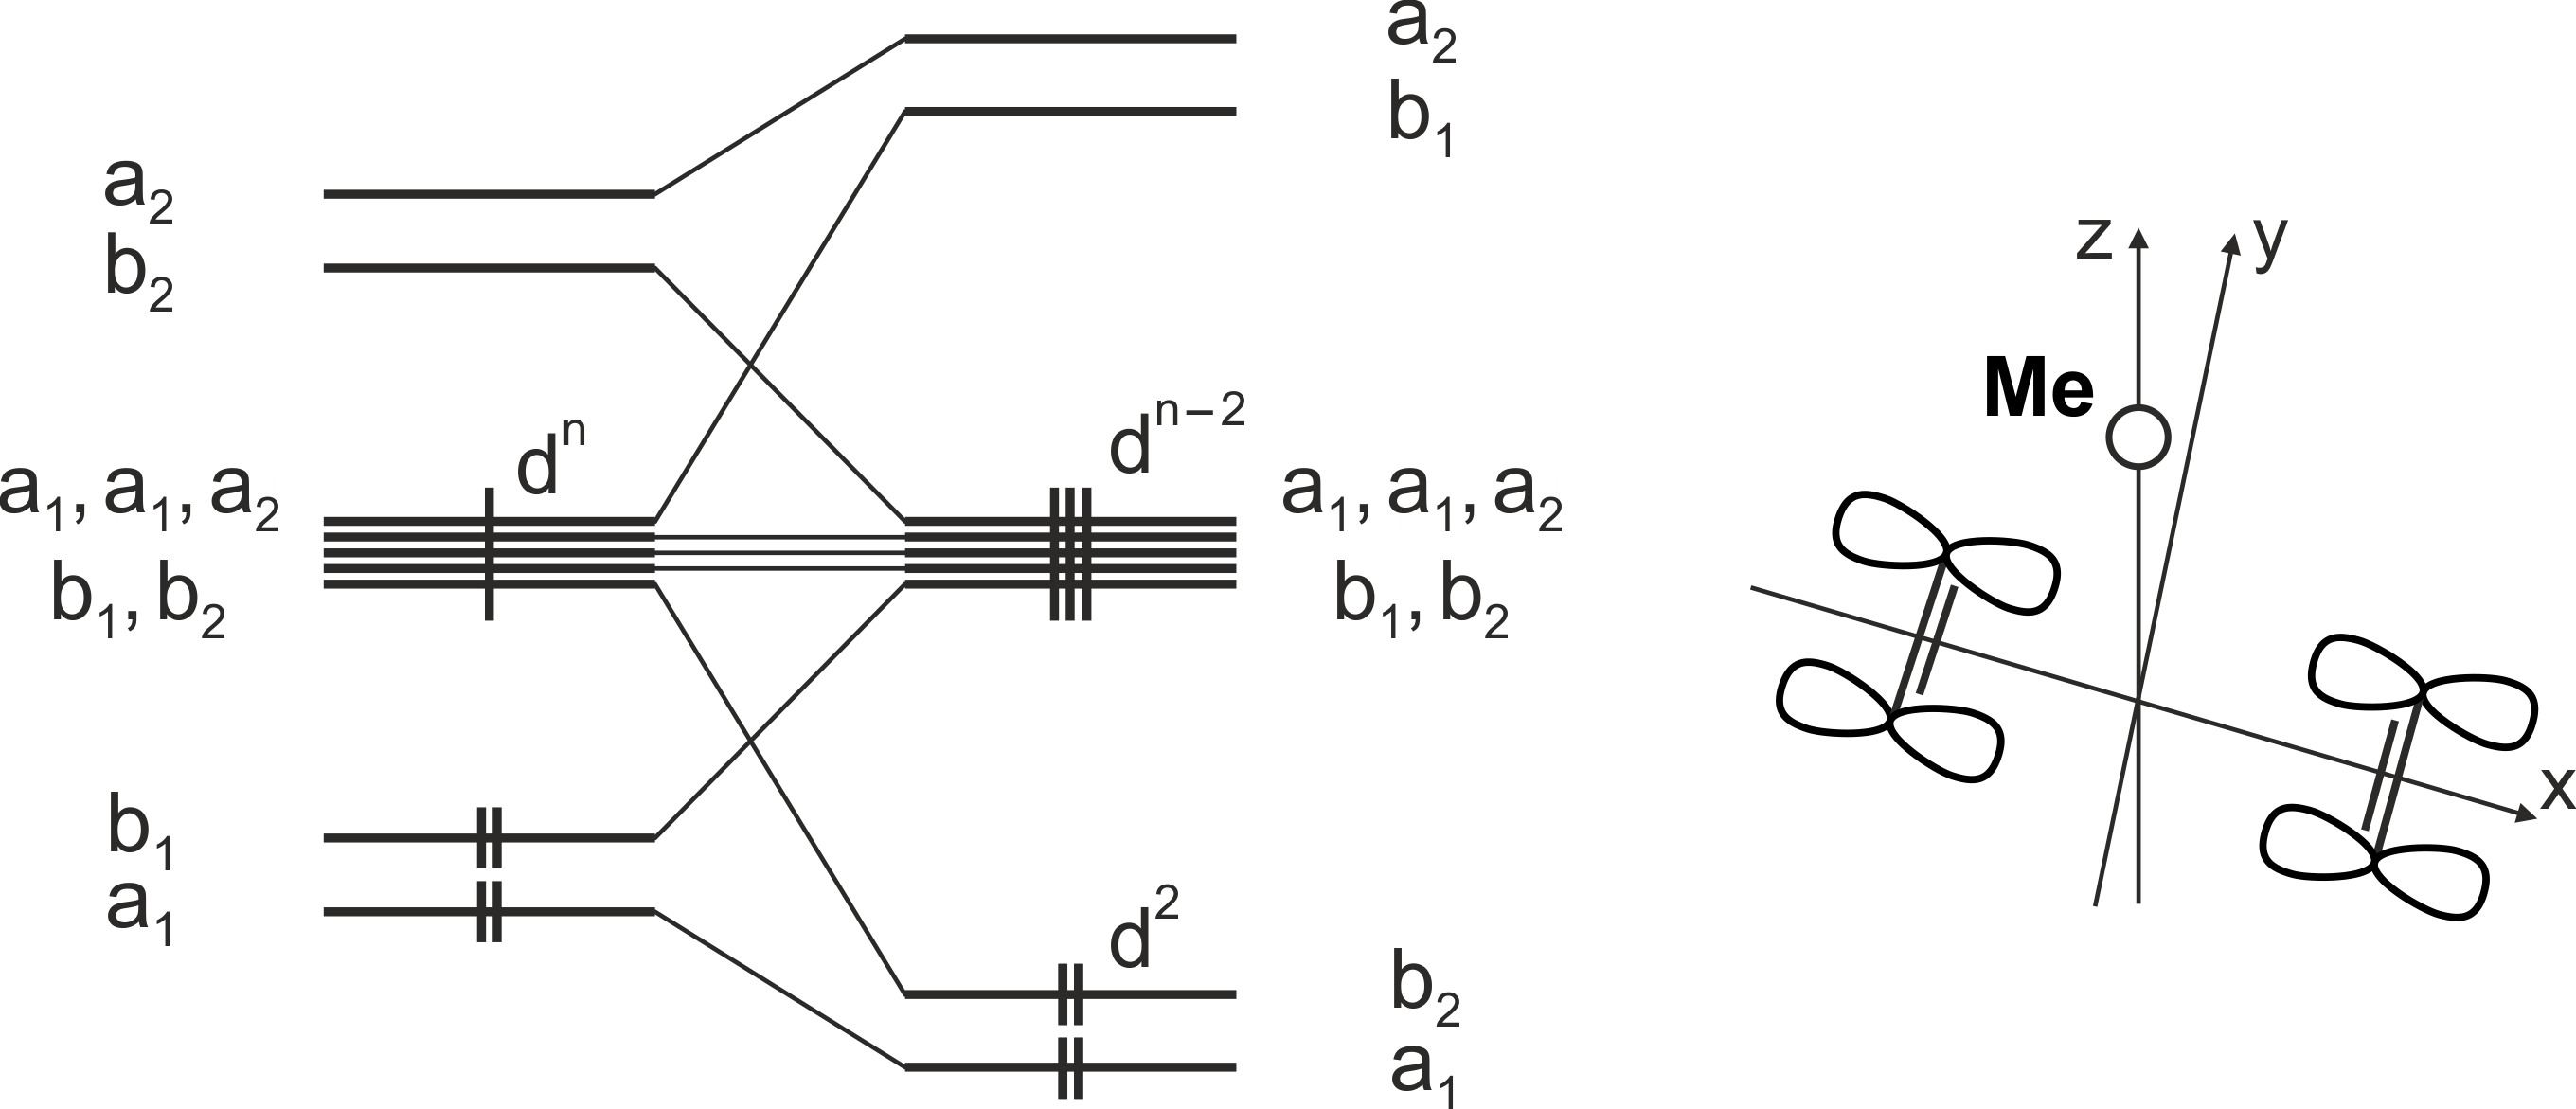
\includegraphics[width=6.5cm]{images/Fig_2_1_12_dec.png}
\centering
\end{figure}
\par
13. Задача 2 контрольной работы 1 весеннего семестра 2024/2025 учебного года. Корреляционная диаграмма для супра-/супра- топологии приведена на~рисунке ниже.
\vspace{-\parskip}
\vspace{1.5mm}
\begin{figure}[h]
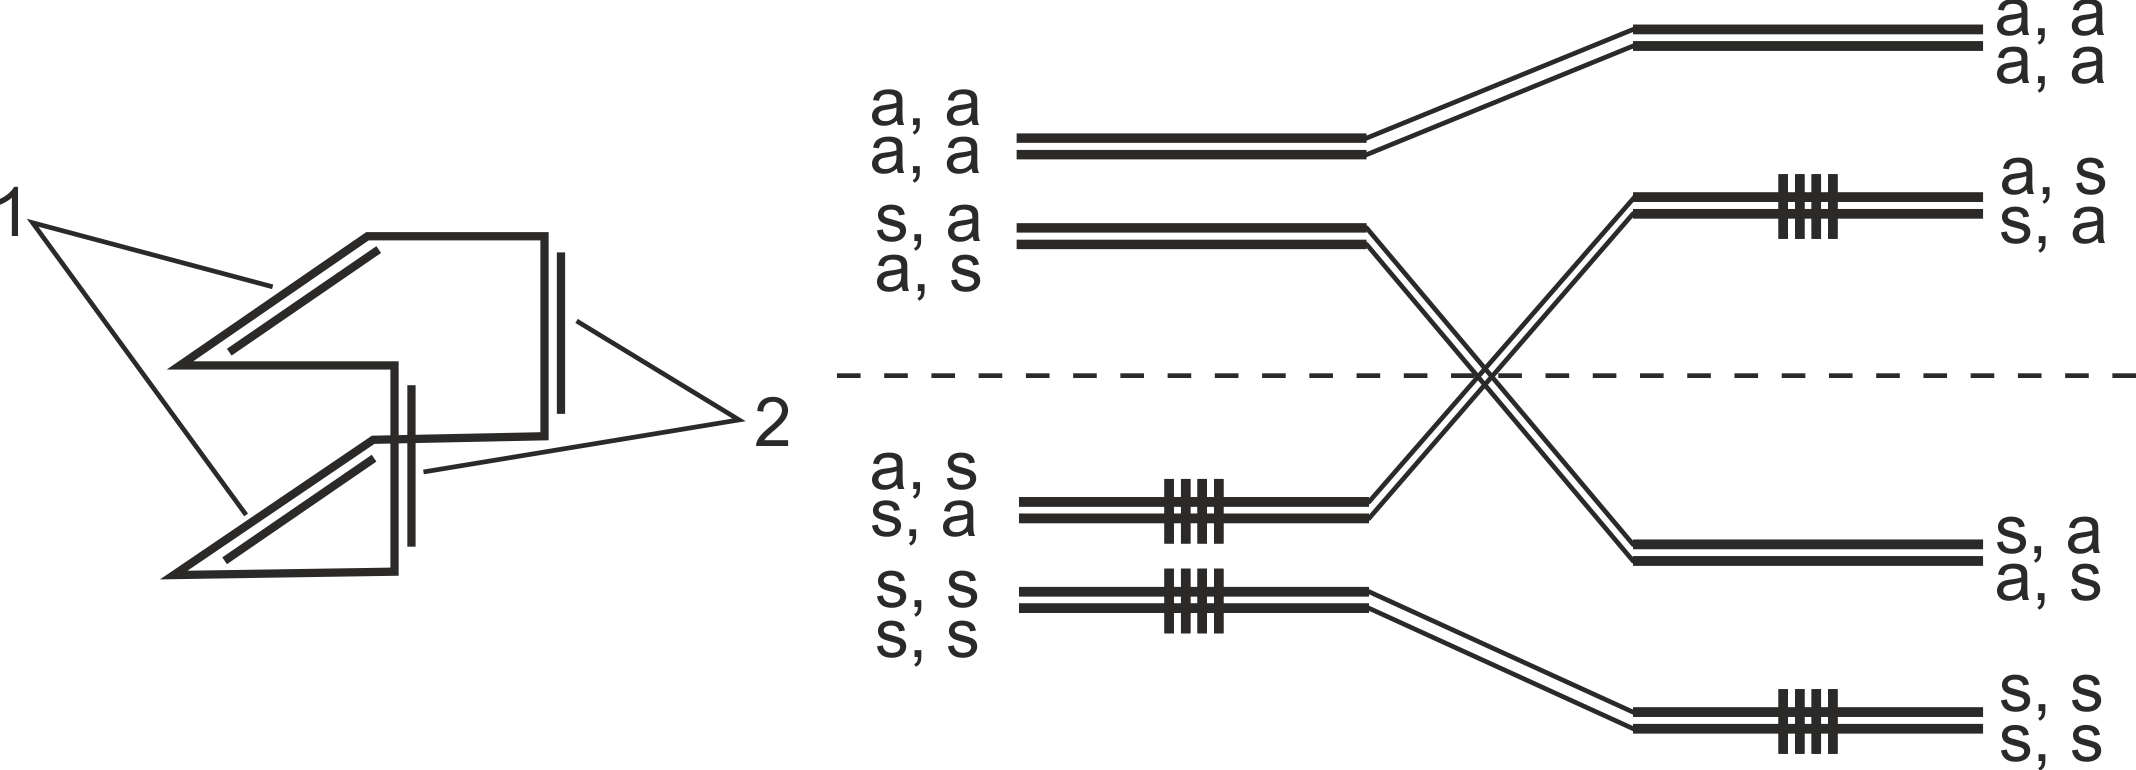
\includegraphics[width=8cm]{images/Fig_2_1_13_dec.png}
\centering
\end{figure}
\par
\vspace{-\parskip}
\newpage

\subsection{Теория кристаллического поля}
1. \\
2. 
\newpage

\subsection{Электронная спектроскопия}
1. \\
2. 
\newpage

\subsection{ИК и КР спектроскопии}
1. \\
2. 
\newpage

\subsection{Эффект Яна-Теллера}
1. \\
2. 
\newpage

\subsection{Вращательная спектроскопия и ее производные}
1. Предел канта равен $\frac{\text{d}}{\text{d}J}( \Delta E_R) = -\frac{1}{2}-\frac{B'}{B'-B}$, где $B'$ и $B$ – вращательные постоянные для колебательных состояний $\nu=1$ и $\nu=0$, соответственно. Подстановка межъядерного расстояния в эту формулу после округления до ближайшего целого числа дает 49.\par
2. $B=6,08114$ ГГц, $I=1,37\cdot10^{-45}$ кг$\cdot$м$^2$. Длины связей определяются из системы уравнений, составленной на основе моментов инерции изотопологов $^{16}\text{O}^{12}\text{C}^{32}\text{S}$ и~$^{16}\text{O}^{12}\text{C}^{34}\text{S}$, посчитанных с помощью приведенных в~условии данных.\par
3. \par
4. Группа симметрии $D_{4h}$, симметрический волчок. $A=B/2$.\par
5. X$-$X$-$Y линейная.\par
6. $J=2k$, $F=0$; $J=2k+1$, $F=1$, где $F$ – полный ядерный спин двух атомов водорода, $k$ – положительное целое число.\par
7. \par
8. \par
9. 25/64.\par
10. \par
11. Задача 2 контрольной работы 2 весеннего семестра 2024/2025 учебного года. $R=1,25\cdot10^{-10}$ м. Молекула HCl имеет приведенную массу, близкую к заданной в условии. \par
12. Задача 2 контрольной работы 2 весеннего семестра 2023/2024 учебного года. $B=3013,845$ МГц, $R=2,17\cdot10^{-10}$ м.\par
13. Задача 2 контрольной работы 2 весеннего семестра 2022/2023 учебного года. В обоих случаях чисто вращательный спектр будет представлять из себя набор эквидистантных линий, с расстоянием между линиями равным вращательной постоянной и относительной интенсивностью, определяемой населенностью вращательных уровней $N_J$. Населенность равна $(2J+1)\exp(-BJ(J+1)/kT)$ и~$(J+1)\exp(-BJ(J+1)/kT)$, соответственно, без учета и при учете описанного в~условии фактора. Анализ показывает, что максимум указанных величин $N_J$~достигается при $J_{max}\approx 2,65$ и $J_{max}\approx 2,41$. Таким образом, максимальной интенсивности будут обадать линии, соответствующие переходам с вращательных уровней $J=2$ и $J=3$.\par
\newpage

\subsection{ЭПР спектроскопия}
1. \\
2. 
\newpage

\subsection{Химический обмен в магнитном резонансе}
1. \\
2. 
\newpage

\subsection{ЯМР спектроскопия}
1. \\
2. 
\newpage
